\section{IP protocol}
IP 프로토콜은 OSI 참조 모델의 제 3계층인 네트워크 계층에서 정의된 패킷 (또는 IP 데이터그램)을 출발지에서 목적지까지 전달하는 기능을 담당한다. 이를 위해 최선형(Best Effort)서비스를 이용한다. 최선형 서비스는 패킷을 목적지까지 확실하게 전달하는 것을 보장하는 것이 아닌, 전송하는데 최선을 다하는 방식이기 때문에 전송 도중에 패킷이 손상될 수 있고, 패킷들이 순차적으로 도착하지 않을 수가 있다. 따라서 IP 프로토콜 고유의 최선형 서비스 특성의 단점을 극복하기 위해서는 상위 계층의 TCP와 같은 신뢰성 있는 프로토콜의 도움을 받아야 한다.
\subsection{IP diagram의 구성}
    \subsubsection*{Version }
    IP가 어떤 버전을 사용하는지를 나타낸다. 현재는 IPv4를 사용하고 있다. 하지만 버전 4의 주소 고갈 문제와 보안 이슈로 인해 IPv6가 등장하게 되었다. v6는 패킷 처리에 대한 오버헤드를 줄이기 위해 v4의 헤더를 대폭 간소화하였으며 128비트의 주소 공간을 가지고 있어 무한대에 가까운 주소를 할당할 수 있고 기존의 v4와 달리 주소의 클래스를 나누지 않고 단순히 유니캐스트(unicast, anycastm multicast)의 주소 형태로 나누었다. v4에는 보안 항목이 없어 보완하기 위해 IPSec와 같은 프로토콜을 사용하였는데 v6는 프로토콜 내에 보안 관련 기능을 가지고 있다.

    \vspace{-4mm}  
    \begin{figure}[!h]\centering
		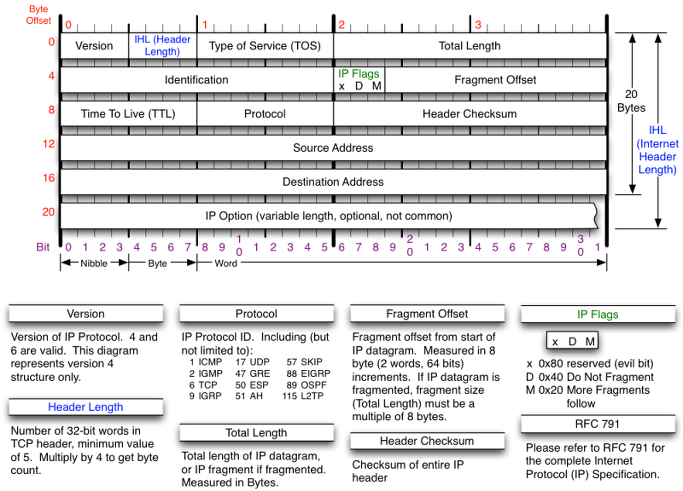
\includegraphics[width=.9\textwidth]{image/week01/3-1-1.png}
		\caption{\small IP Header Diagram}
		\vspace{-10pt}
    \end{figure}
   \vspace{-4mm}  
    
    \subsubsection*{TOS (Type of Service)}
    ToS는 우선쉰위를 나타내는 3비트의 Precedence 및 4비트의 서비스 유형 지정 비트, 그리고 사용되지 않은 1비트이다. ToS 필드를 사용하여 라우터나 호스트 등의 장치에서 패킷 처리에 대한 우선순위(QoS)를 설정할 수 있는데 현재는 DSCP(Differentiated Serviecs Code Point) 필드로 정의되어 있다.
    \vspace{-1mm}
    \subsubsection*{Total Length}
    ToS는 우선쉰위를 나타내는 3비트의 Precedence 및 4비트의 서비스 유형 지정 비트, 그리고 사용되지 않은 1비트이다. ToS 필드를 사용하여 라우터나 호스트 등의 장치에서 패킷 처리에 대한 우선순위(QoS)를 설정할 수 있는데 현재는 DSCP(Differentiated Serviecs Code Point) 필드로 정의되어 있다.
    \vspace{-1mm}
    \subsubsection*{Identification}
    생성되는 각각의 패킷마다 부여된느 고유의 번호이다. 패킷은 제 2계층 프로토콜의 최대 전송 단위(MTU) 값에 따라 여러 개의 프로그먼트(Fragment)로 분할되어 처리되는데, 분할되어 온 fragment들을 원래의 패킷으로 재조립할 때 이 식별자 값을 기준으로 한다.
    \vspace{-1mm}
    \subsubsection*{Flags}
    IP 패킷의 분할\footnote{fragmentation} 가능 여부와 마지막 fragment인지 아닌지를 알리기 위해 사용되는 필드이다.
    \vspace{-1mm}
    \subsubsection*{Fragment Offset (분할위치)}
    하나의 패킷이 여러 개의 프래그먼트로 분할될 때, 각각의 프래그먼트 내의 페이 로드가 원래의 패킷 내의 페이로드를 기준으로 어떤 위치에 있는지를 명시하는 필드이다. 따라서 분할된 프레그먼트들은 이 분할 위치 값을 이용하여 원래의 패킷으로 재조립되게 된다.
    \vspace{-1mm}
    \subsubsection*{TTL (Time to Live)}
    패킷의 루핑 현상으로 인한 문제를 해결하기 위해 사용하는 필드로 패킷의 수명을 나타낸다. 예를 들어 TTL값은 라우터를 1개 지날 때마다 2씩 감소되어 이 값이 0 이 되면 해당 패킷은 네트워크에서 폐기된다.
    \vspace{-1mm}
    \subsubsection*{Protocol}
    패킷의 캡슐화되어 있는 상위 계층 PDU가 어떠한 프로토콜을 사용하는지를 명시하는 필드이다. 예를 들어 캡슐화된 PDU가 TCP 세그먼트일 경우 이 필드는 6의 값을, UDP 세그먼트일 경우에는 17의 값을 갖는다.
    \vspace{-1mm}
    \subsubsection*{Head Checksum}
    P 헤더의 오류 검사를 위한 필드이다. TCP와 UDP를 포함하여 IP 데이터그램으로 캡슐화되는 프로토콜은 대부분 헤더 및 데이터를 포함하는 체크섬 필드를 가지고 있기 때문에 IP 데이터그램의 체크섬 필드는 단순히 IP 헤더에 대한 오류 검사만을 수행한다.
    \vspace{-1mm}
    \subsubsection*{Source IP Address }
    32비트 길이의 출발지 장치의 ip 주소이다. ip 주소는 네트워크 필드 및 호스트 필드의 길이에 따라 클래스 a, 클래스 b, 클래스 c 주소로 나뉜다. 이 외에도 클래스 D 및 클래스 E 주소가 있지만, 이는 각각 멀티캐스트 주소와 예약된 주소로서 네트워킹 장치나 호스트에 할당하는 주소는 아니다.
    \vspace{-1mm}
    \subsubsection*{Destination IP Address}
    32비트 길이의 목적지 장치의 IP 주소이다.
    \vspace{-1mm}
    \subsubsection*{Options}
    패킷의 전송 경로를 포함한 IP 프로토콜의 동작 옵셥을 정의하는 필드이다.